\frame { \frametitle{Monte Carlo Method}
Monte Carlo methods are the only practical choices to do very high dimension integrations such as 
equation~\ref{partition_function}.

For $x \in\mathcal{C}$ with weight $p(x)$, we have the partition function
\begin{equation}
Z=\int_{C} dx~p(x)
\end{equation}

The expectation value of a quantity A is given by
\begin{equation}
 \langle A \rangle_{p} = \frac{1}{Z}\int_{C} dx~A(x)p(x)
\end{equation}

With $M$ configurations $x_i$ in a Monte Carlo procedure,

\begin{equation}
\langle A \rangle_p \approx \langle A \rangle_{MC} \equiv \frac{1}{M}\sum_{i=1}^M {A}(x_i).
\end{equation}

}

\frame { \frametitle{Markov Process}

A Markov process defines a transition matrix $W_{xy}$ which specifies 
the probability to go from state $x$ to state $y$ in one step of 
the Markov process.

The Markov process will converge exponentially from any initial state to a stationary distribution $p(x)$ 
if two conditions are satisfied.
\begin{block}{}
\begin{itemize}
\item Ergodicity: for all $x$ and $y$ there exists an integer $N<\infty$ such that for all $n\ge N$ the probability  $(W^n)_{xy}\ne 0$.
\item Balance: the distribution $p(x)$ satisfies the detailed balance condition
\begin{align}
\frac{W_{xy}}{W_{yx}} = \frac{p(y)}{p(x)} \nonumber
\end{align}
\end{itemize}
\end{block}
}

\frame { \frametitle{Metropolis-Hastings Algorithm}
An update from a configuration $x$ to a new configuration $y$ is proposed with a probability 
$W_{xy}^{\text{prop}}$ but accepted only with probability $W_{xy}^{\text{acc}}$.  
If the proposal is rejected  the old configuration $x$ is used again.

\begin{equation}
 W_{xy}^{\text{acc}}= \min\left[ 1,  \frac{p(y) W_{yx}^{\text{prop}}}{p(x) W_{xy}^{\text{prop}}} \right].
\end{equation}
\begin{align}
W_{xy} &= W_{xy}^{\text{prop}}W_{xy}^{\text{acc}}
\end{align}
}

\frame { \frametitle{Hybridization Update Diagrams}
(a) original configuration; (b) removal of a segment; (c) shift of an end point of a segment; (d) insertion of an antisegment; (e) removal of an antisegment; (f) removal of another antisegment such that the remaining segment "wraps" around $\beta$.
\begin{figure}
    \begin{center}
      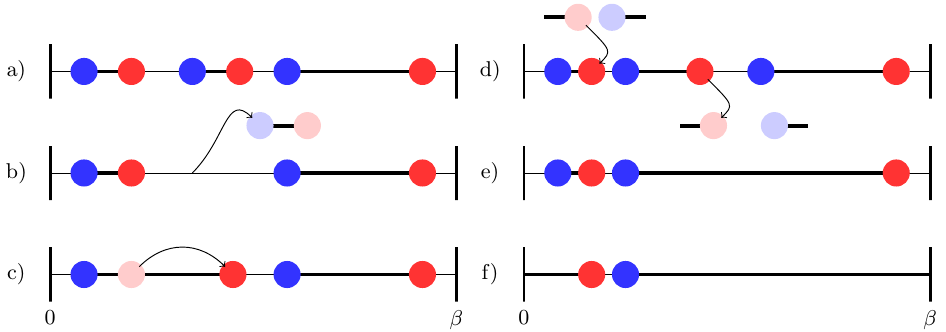
\includegraphics[width=0.95\textwidth]{hyb_diagrams.png}
    \end{center}
  \end{figure}
}

\frame { \frametitle{Segment Representation}
Segment representation make it possible to treat interaction by looking at overlap of lines.
Extension to density - density interactions for multiple orbitals
is made straightforward as well.
\\
\begin{figure}
    \vspace{20pt}
    \begin{center}
      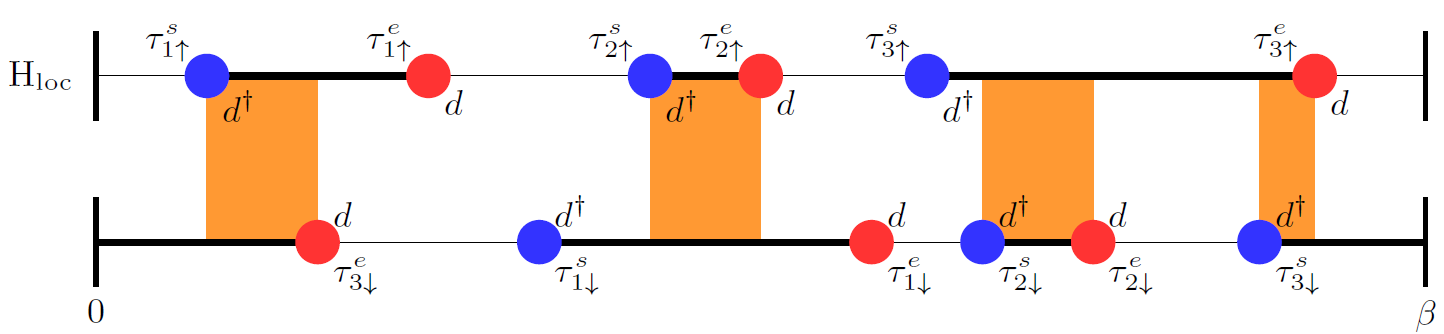
\includegraphics[width=0.95\textwidth]{segment}
    \end{center}
  \end{figure}
}

\frame { \frametitle{Segment Representation}
Possible hybridization lines of a particular segment configuration.
\\
\begin{figure}
    \begin{center}
      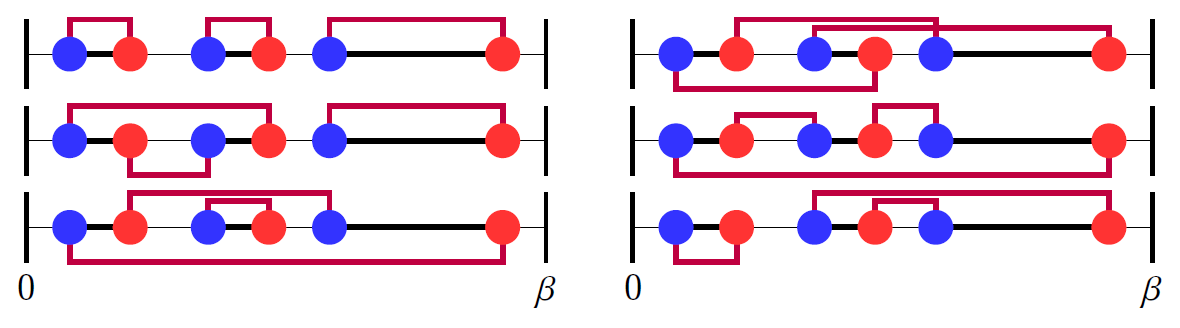
\includegraphics[width=0.9\textwidth]{hybridization_lines}
    \end{center}
    \vspace{-20pt}
  \end{figure}
}


\frame { \frametitle{CTQMC Workflow}
  \begin{figure}
    \begin{center}
      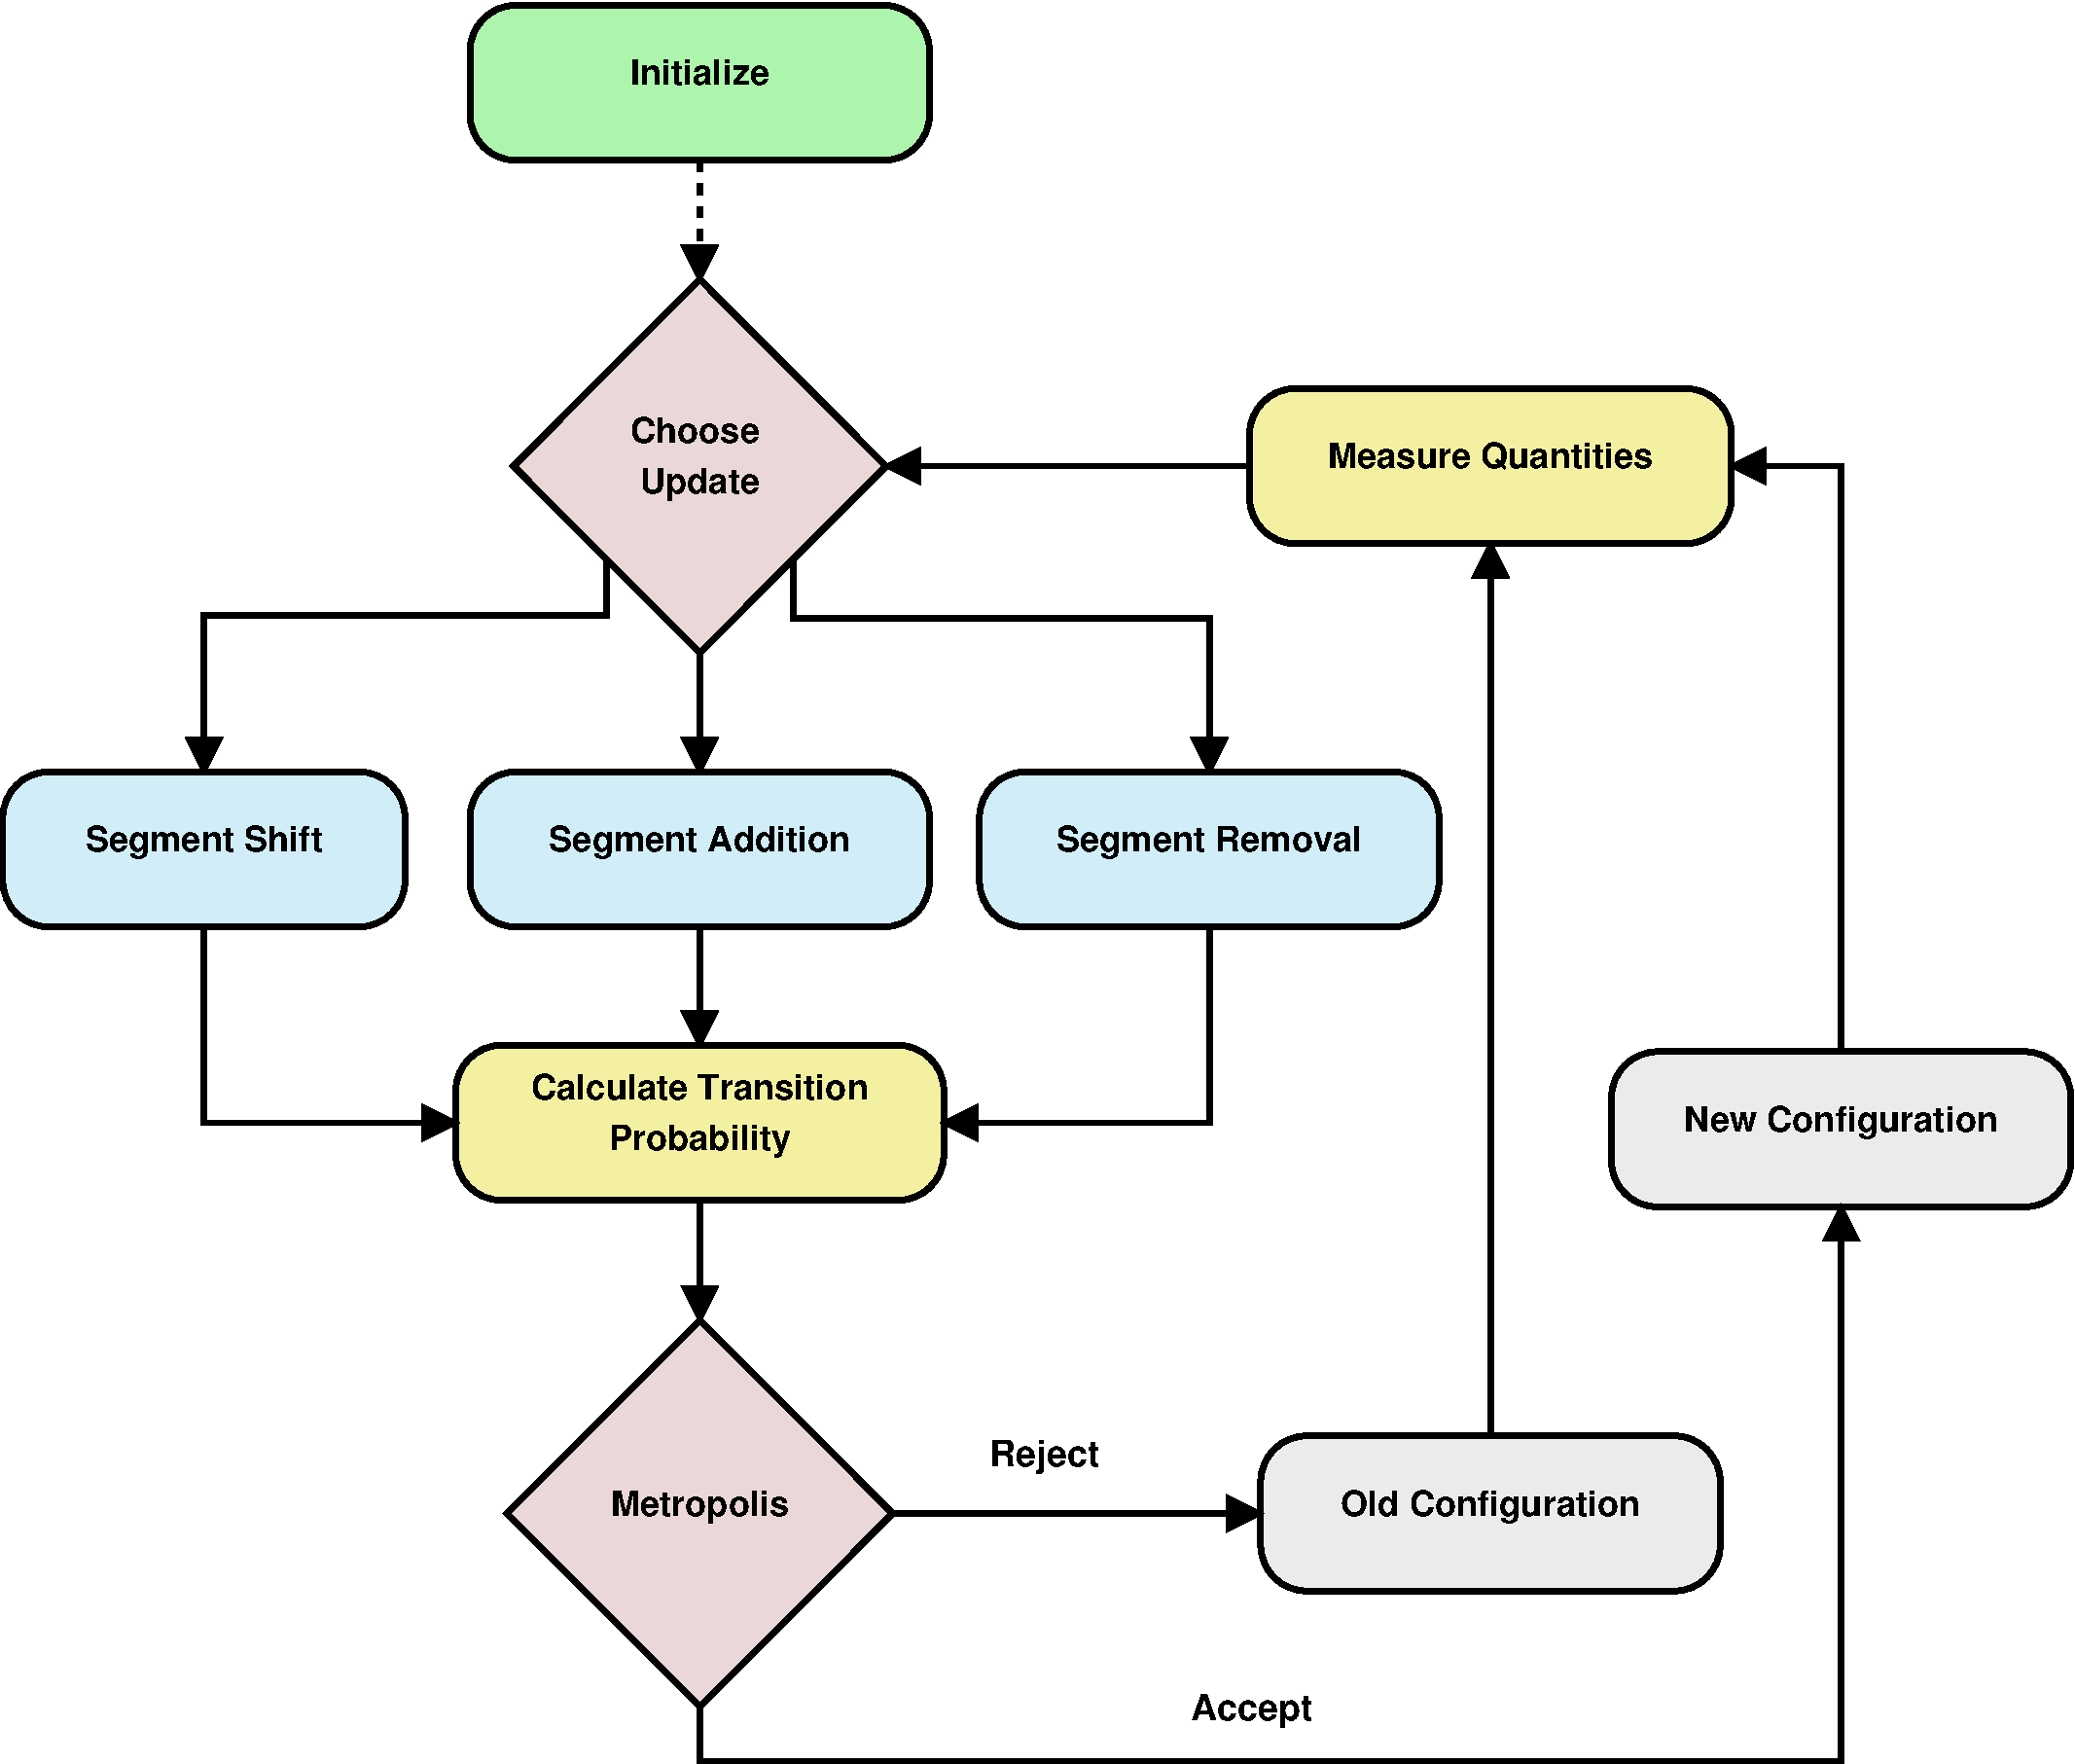
\includegraphics[height=0.7\textwidth]{CTQMC}
    \end{center}
  \end{figure}
}